%!TEX program = xelatex
\documentclass[a4paper]{ctexart}

\usepackage{listings} 
\usepackage{geometry}
\usepackage{booktabs}
\usepackage{graphicx}
\usepackage{tabularx}
\usepackage{multirow}
\usepackage{enumitem}
\usepackage[bottom]{footmisc}
\usepackage[table,xcdraw]{xcolor}

\renewcommand{\multirowsetup}{\centering}

\geometry{
    left=23mm,
    right=23mm,
    top=23mm,
    bottom=23mm,
}

\setlength{\parskip}{0.5em}

\title{\Huge PetLover 商业计划书}

\author{
  项目成员:\\
  姬筠刚 191250055(PM)\\
  陈梓俊 191250016\\
  丁炳智 191250024\\
  刘庭烽 191250093\\
}
\date{\today}

\begin{document}

\maketitle

\centerline{
\includegraphics[]{logo.png}}

\newpage

\tableofcontents

\newpage

\setlength{\parskip}{1em}

\begin{abstract}
  本项目名为PetLover,是由PetLover小组于2021年秋季学期《需求与商业模式创新》课程大作业中设计的软件产品项目。此文档为商业计划书,主要内容包含项目简介、市场与竞争分析、主要产品介绍、财务分析、运营规划、风险预测及分析方案和团队介绍。
  
  本创业计划书属于商业机密,其所涉及的内容和资料只限于PetLover团队成员使用。收到本创业计划书后,收件人应遵守以下规定:
\begin{enumerate}
  \item 本创业计划书仅限于本次课程作业规定人员使用;
  \item 在没有取得本创业团队的书面同意前,不得将本创业计划书全部和或部分复制、影印、泄露或散布给他人。
\end{enumerate}
\end{abstract}


\section{项目简介}

\subsection{项目背景}
宠物,是当代社会人群必不可少的陪伴,无论是在外打拼的年轻人群体,还是安度晚年的老年人群体,抑或是中年人群体,都对宠物饲养有着或多或少的要求。由此,一些宠物交易市场和宠物日常交流平台应运而生。

经过一段时间的市场调研,我们发现:虽然目前市场上已存在宠物交易平台和宠物成长分享平台,但是能够提供一站式宠物服务(包括从宠物买卖、宠物饲养交流、宠物用品到宠物日常分享等的一系列相关服务)的软件平台少之又少。用户往往需要在平台A进行宠物交易,在平台B进行宠物用品购买,在平台C进行宠物疾病咨询,在平台D分享宠物日常……

为了避免宠物主人在各个平台之间“反复横跳”,我们计划打造一款集宠物(及相关用品)交易、宠物疾病咨询、宠物饲养教程、宠物日常分享四大功能于一身的宠物交流平台——PetLover平台(以下简称“PetLover”或“平台”),希望通过一站式服务真正地为宠物爱好者们提供便利;同时通过与各地线下实体宠物店、宠物医院等进行合作,建立全国各地的宠物交易/问诊线下网络,推进线上、线下双线模式的宠物交易和宠物疾病诊疗服务。

PetLover,帮助宠物爱好者们从头见证宠物宝贝的成长!

\subsection{项目结构总览}
PetLover项目是面向整合宠物买卖、宠物饲养交流、宠物用品、宠物日常分享交流社区等服务于一体建立一站式服务平台的项目,项目结构将按照主营业务、增值服务、未来服务布局展开。

\subsubsection{主营业务}
\paragraph{1、宠物社区的建立与维护:}PetLover项目的核心是社区,我们将建立一个宠物饲养交流、宠物知识分享及动物保护理念宣传的社区平台,社区为PetLover用户智能化推荐浏览内容,用户可以按照话题查看帖子,也可以针对某些内容进行创作。
\paragraph{2、宠物商城的维护与推广:}PetLover平台提供宠物商城服务,包括宠物购买、宠物用品购买及宠物服务购买等服务,为用户提供商品质量保证,并以完善的供应链渠道为用户提供良好的购物体验。
\paragraph{3、宠物医疗的咨询与服务:}PetLover平台提供宠物健康论坛及服务平台,通过宠物健康知识分享、宠物健康咨询、宠物线上问诊、宠物医疗线上预约、宠物药品配送等服务来帮助宠物主人保障爱宠的健康,与各地宠物医院签约并推行该平台作为宠物医院线上问诊的主要平台,为宠物健康撑起一个强有力的保护伞。
\subsubsection{增值服务}
\paragraph{1、铺设线下网点:}PetLover项目在各地加盟线下宠物服务网点,为辐射区域内的用户提供宠物的一系列服务,包括宠物生活服务、宠物医疗服务、商品配送服务等等,每个线下网点提供的服务范围可以有所不同,网点经营者可以根据需要自由选择。
\paragraph{2、动物保护:}PetLover平台将在社区设立动物保护宣传板块,本平台将获得动物保护组织(如中国小动物协会)的许可和授权,吸引动物保护组织成员和自媒体入驻社区论坛,宣传动物保护思想,贯彻珍爱生命、倡导精神文明和发扬人道主义精神的理念,提升企业竞争软实力。
\subsubsection{未来服务布局}
PetLover平台未来将朝向以下几点服务布局前进:
\paragraph{1、宠物社区和商城基准高质量:}平台对社区内容和电商模块进行严格质量把关,社区论坛内容需要经过二级审核(审核人员审核和平台管理员抽查审核),尽可能使内容不含不良信息和垃圾广告等;电商模块与合作的商家与机构签订商品与服务质量保证协议,严格审核商品质量;平台内节制广告宣传,合理而正确地规划广告位,追求原生广告和创意广告。PetLover 为用户提供可靠干净的社区环境。
\paragraph{2、加强基础设施建设:}PetLover在项目初期很难拥有实体资源,度过项目初期后首要目标是加强基础设施建设,以扩大平台影响力,其具体做法是建设线下服务网点并扩大每个线下服务网点的服务范围。
\paragraph{3、持续贯彻动物保护理念:}贯彻动物保护理念是平台的生命力所在,PetLover平台未来将继续扩展动物保护这个关键业务的活动范围,将我们的动物保护志愿者的客户细分提升为动物保护组织成员,同时将中国小动物保护协会/动物保护志愿者的重要合作拓展为动物保护组织及其成员。同时强调了合作成本作为动物保护的经济支撑。

\subsection{产品简介}
PetLover是一款专注于为养宠者提供一站式综合服务的产品,它将为养宠者提供宠物交流社区、宠物百科、宠物/用品/服务在线购买、宠物健康问题在线咨询等服务。PetLover平台致力于解决养宠用户:养宠点滴无法分享、养宠知识难以获取、宠物生病手忙脚乱等痛点,将现有宠物相关知识资源、实物资源、人力资源等以平台形式进行有机整合,充分发挥宠物行业各要素的作用,降低用户使用困难,切实解决用户痛点。此外,平台将通过社区等渠道宣传宠物保护理念、组织宠物保护展、推广动物保护思想乃至开展流浪宠物领养等,实现产品的社会价值。

\subsection{市场情况}
\subsubsection{宠物消费市场处于快速发展阶段}
我国宠物行业从20世纪90 年代初的花鸟市场年代,伴随着宠物消费产品和服务的日益丰富、人口结构的变化、宠物角色和养宠理念的转变、以及移动互联网技术对宠物行业交易模式和服务模式的改变,经过30 年的发展,我国宠物行业经历了启蒙期、孕育期、发展期,目前进入了有序增长的高速发展期。根据中国宠物行业白皮书,2019年中国城镇宠物消费市场规模答2024亿元,同比增长18.5\%。2020年中国宠物经济产业规模达2953亿元,同比增长33.5\%。受政策、经济、社会和技术因素驱动,以及疫情带来的更多潜在养宠人群及情感消费,未来三年宠物行业将继续 保持平稳增长 ,复合增速预计14.2\%,到 2023 年行业规模将达到 4456 亿元。
\subsubsection{宠物食品市场是核心,医疗、日用品、各形态服务日渐丰富}
宠物行业产业结构中,宠物食品类目是宠物行业最大的细分市场,随着人们对喂养商品粮的认知提升,市场对宠物食品的需求将进一步释放;其次是宠物医疗,主要为依托宠物医院和个体诊所的诊疗服务;宠物用品的细分品类较多,其中智能设备的成交量快速增长;宠物服务的形式日渐丰富,随着居民消费升级和养宠理念、宠物角色的转变,宠物服务行业将稳步增长。
\subsubsection{养宠人群向低线城市下沉,养宠人群扩大}
根据中国宠物行业白皮书显示,养宠人群向低线城市下沉,一线城市宠物主人占比38.8\%,二三线城市也不容小觑。同时一线城市90后、95后占比更高,分别为49.8\%和50.1\%,一线城市的养宠人群更加年轻化。同时养宠人群不断扩展,越来越多高学历、中高收入人群开始养宠。大学本科及硕士以上学历的宠物主人占比分别增长了2.5\%和2.0\%;同时,收入4000元以上的宠物主人占50.4\%,其中月收入超过1万元的人群占比超过20\%。养宠人群在逐渐大众化的同时,也在趋于高学历和高收入化。
\subsubsection{政策规范、经济发展、人口结构变化及技术进步共同助推行业发展}
国家规范性文件和养宠相关政策条例的陆续推出,推动宠物行业的规范化发展。随着居民收入的提升,居民消费观念升级,重视对生活品质及对情感消费的投入将推进宠物行业消费向多样化发展。人口结构的变化,空巢老人和空巢青年人群的增加,越来越多的人将陪伴的渴望寄托于宠物。同时,新媒体技术的进步,短视频等社交媒体的爆发,驱动了“云吸宠”的发展,为宠物行业带来了更多的市场规模和潜在消费者。

\subsection{商业模式}

PetLover属于多边平台商业模式。多边平台将两个或更多独立但相互依存的客户群体连接在一起。这样的平台对于平台中某一群体的价值在于平台中其他客户群体的存在。平台通过促进不同群体间的互动而创造价值。一个多边平台的价值提升在于它所吸引的用户数量的增加,这种现象被称为网络效应。

PetLover商业模式的核心就是它的价值主张:一站式服务。它使宠物爱好者能够与宠物用品及用品供应商、宠物医疗行业从事者等紧密连接。这些客户群体中的每一个都有各自的价值主张和各自的收益流。而且,这些客户群体之间相互依存,哪一个也无法独立存在。而PetLover的价值主张创造的价值体现在以下三个方面:第一,吸引用户群体;第二,将客户群体进行配对;第三,通过平台提供的交易渠道降低交易成本。

PetLover的核心资源是平台,该平台的强大之处在于,它为养宠者提供一个集成了宠物交流社区、宠物百科、宠物/用品/服务在线购买、宠物健康问题在线咨询等功能于一身的平台,这些服务大大提高了用户粘性。作为一个多边平台,PetLover从宠物爱好者中赚钱,对于另外几个客户群体——宠物用品及用品供应商和宠物医疗行业从事者则提供补贴。越多人使用PetLover,为宠物用品及用品供应商和宠物医疗行业从事者创造的价值就越大。

具体商业模式画布如下:

\begin{center}
  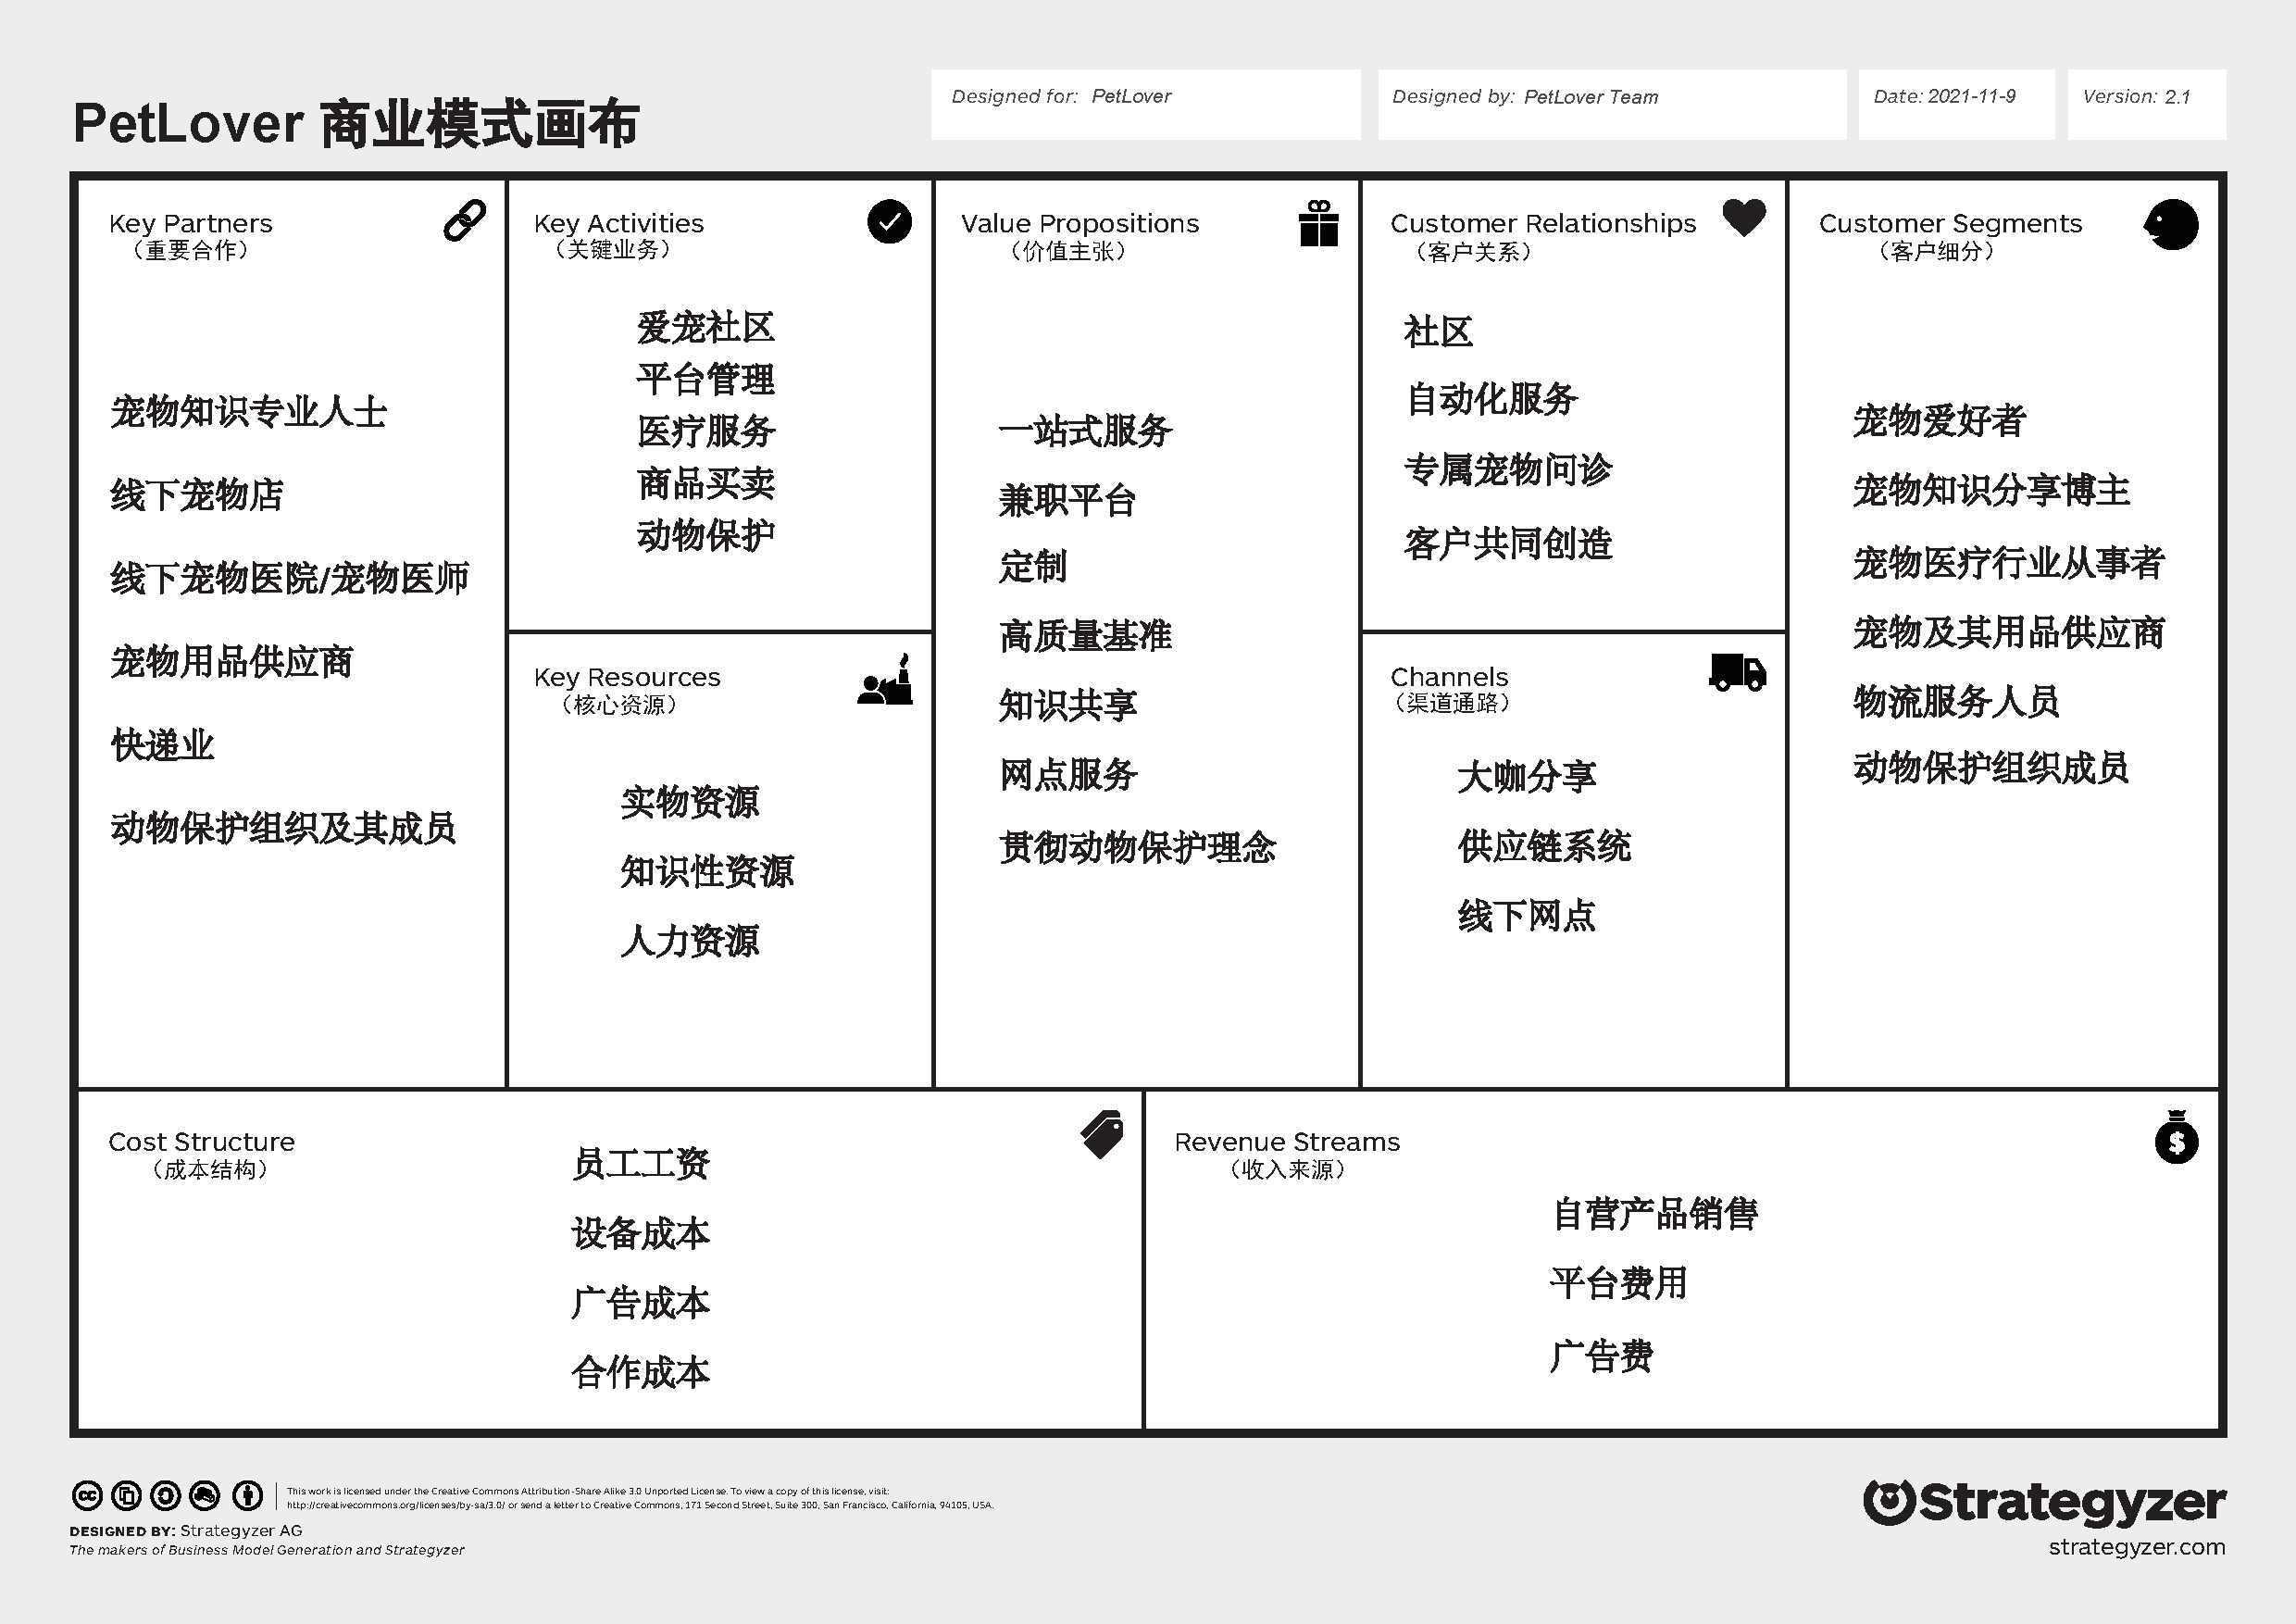
\includegraphics[scale=0.4]{改动后画布.pdf}
\end{center}

\subsection{财务预测}

PetLover项目预计初期启动资金为200万,力求投入第一年即获得高收益,其投入运营后第一至五年资产、负债、收益预测表详见财务分析的财务预测部分。

\section{市场与竞争分析}

\subsection{市场环境}

\subsubsection{市场影响力:宠物市场在不断扩张与独立}
我国经济的快速发展,带动了不少行业,宠物业拥有着庞大的市场,养宠人士每年不断的增加,可以确定这个行业的未来是不可估量的;可以预测未来宠物市场发展将会整合宠物医疗服务、宠物生活服务、宠物网络社区为一体,为现在还在跨平台的用户提供极大的便利,并在这三项服务上做到可靠、优质,另外随着养宠群体的不断扩大,宠物市场在“互联网+”时代很有可能从各大综合平台(如微博超话、Bilibili 动物圈等)独立出来成为一个崭新的平台,而不单单作为一个子平台存在。
\subsubsection{行业影响力:PetLover融合多项服务}

根据我们的市场调研,我们得知除了一些从概念出发的产品以外,目前国内主流的综合宠物服务平台是波奇网、E 宠商城、狗民网、宠物家,他们分别属于宠物服务类的前4 名。其中波奇网、E 宠商城绝对是宠物服务领域的头部玩家。

狗民网现在已经停止运营,我们暂不进行讨论。波奇网的产品主要有客户端的网站以及移动端的波奇宠物,E 宠有客户端的网站E 宠商城以及移动端的E 宠。与现有的在线社交购物平台淘宝京东等相似。波奇网和E 宠商城的优势都是进入宠物服务市场早,在宠物综合服务领域深耕多年,有早期积累起来的经验以及口碑优势,已经经历了多轮融资,与宠物行业上游企业建立起了稳定的合作伙伴关系。宠物家直营线下宠物门店,以社区+ 商城+O2O 的创新商业模式,提供线上线下的一站式服务,其致力于为养宠人群提供高质便利的“平价服务”与“平价商品”。

上述宠物服务平台均无法覆盖社区论坛、医疗服务、商品买卖、线下网点等服务为一体,因此PetLover平台的竞争优势仍然存在,但仍然要注意宠物自媒体可以作为宠物社区的替代品,许多宠物自媒体坐拥众多宠物爱好者流量,给我们的宠物社区带来了巨大的风险威胁。

\subsubsection{关键趋势:多方趋势促进宠物市场扩张}

技术方面,对于购物类/社区类软件来说,软件开发中非常重要的技术就是服务端的部署,并且随着用户数量的不断增加,就需要面临从一百个到数万级甚至千万级并发情况下服务段架构的优化问题。当下,云平台具有成本低、优化性能、规模大等诸多优点,充分利用云端资源进行服务端开发,把海量机器资源通过统一的资源平台进行管理,已是这类软件技术发展的必然趋势。

监管法规方面,随着互联网的发展,国家对虚拟网络的监管力度不断增大。社区中所有帖子和言论都不能有非法的情况发生,加强社区监管是平台发展中的一项重要工作。我们需要约束社区用户自觉以国家安全为重,规范自己在社区中的言论,这样的管理有利于社区保留更有价值的观念,减少争论和舆论的酝酿发展。对于平台的购物板块来说,平台运营过程中要对商家进行管理,保证商品的质量和合理定价,并要求商家给出完善的交易规则。对于可能存在的部分商品虚假宣传,平台需要给予警告和下架;同时,平台需要建立完善的客服制度,让消费者找得到商家、找得到平台;对于消费者的投诉,我们也必须认真对待,不断反思,建设更加完善的购物流程体系。

社会文化方面,饲养宠物已经成为当代中国社会文化中十分重要的一部分,在生活节奏不断加快的今天,年轻人、中年人终日疲于维系生活,并且随着社会结构的不断变化,空巢群体不断增加,宠物逐渐成为人们的精神寄托和情感慰藉。通过饲养宠物缓解孤独、舒缓压力、填补感情。在这样的社会大背景下,我们平台应运而生,采取顺应时代的商业模式,为消费者提供优质的宠物服务,把健康活泼的宠物送到爱宠人士身边,给他们带来情感慰藉和贴心服务。

社会经济方面,国内少子家庭、丁克家庭增多,人口老龄化加快,空巢青年、老人数量增长,是我国宠物饲养数量快速上涨的主要原因;从养宠人群收入状况来看,低收入人群的养宠比例较高,说明养宠活动也在逐渐大众化。

\subsubsection{宏观经济影响:国家政策与互联网共同推动宠物行业}

在互联网浪潮的席卷之下,线上经济的蓬勃发展为宠物经济的壮大提供了巨大便利,宠物服务平台出现在大众视野当中,而后诸如共享经济、云养宠等新型服务模式也日益兴起。整体而言,我国处在宠物行业发展的黄金时期;而且宠物行业的资本市场目前十分火爆。目前宠物行业仍处于高速增长期,增速仍将保持在20\% 以上,此外当前宠物行业实物资源增长也较快。国持续深入推进“互联网+”行动,加快数字经济创新发展试验区建设,积极运用中央预算内投资等各方面资金,加强包括5G、数据中心、工业互联网等新型基础设施建设,推进大数据、云计算、人工智能、物联网等技术的集成创新和融合运用,加快培育一批吸纳就业能力强的数字经济产业,加快改造传统产业,促进平台经济、共享经济持续健康发展,培育更多的经济和就业新增长点。这将为PetLover 平台的建立提供坚实的基础设施保障,同时也让平台有能力成为用户与线下网点的中间节点。

\subsection{目标市场与需求分析}

\subsubsection{目标市场}

饲养宠物已经成为当代中国社会文化中十分重要的一部分,在生活节奏不断加快、空巢青年/老人群体数量不断增加的大背景下,人们往往会选择通过饲养宠物来缓解孤独、舒缓压力、填补感情。平台的目标市场也是国内的“丁克”家庭、空巢青年、空巢老人,并根据市场调研,女性养宠比例及90后养宠人群占比较大,这类人群是平台重点关注的目标用户群体。

\subsubsection{需求分析}

对于欲养宠人群或养宠新手人群来讲,在初次接触宠物饲养时,由于缺乏经验,他们需要在多个平台之间反复切换,以寻求养宠攻略,且网络中虚假信息和冗余信息较多;此外,他们分享宠物日常的途径较少,随之得到的反馈也较少;欲购买宠物用品时,由于购买渠道纷杂也难以保证用品的质量;并且在宠物需要进行诊疗时,寻求宠物医疗服务需要耗费大量成本。

因此,对于计划养宠和初次接触养宠的用户来说,他们希望能够有一个线上平台,能够全方位地了解各种宠物的特征信息并能更加划算、可靠地购买宠物/用品及服务;对于拥有宠物的用户,他们深受虚假信息和广告信息的困扰,希望有可靠专业的渠道获取养宠知识,同时也希望分享自己爱宠的动态以获得他人的肯定和情感的共鸣;同时他们希望降低宠物饲养的成本、购买便宜高质量的宠物用品、方便快捷地为爱宠寻求医疗服务和日常服务;对于不养宠的用户来说,他们也可以通过浏览平台的社区进行“云吸宠”,看到其他用户的宠物分享来得到精神上的慰藉。

\subsection{市场规模}
宠物行业的市场目前十分火爆,目前宠物行业仍处于高速增长期,增速仍将保持在20\%以上,是一个千亿级赛道。

我国宠物行业发展自20世纪90年代初开始,到如今大致经历了四个阶段,从最初的初具规模期,到20世纪90年代末的快速发展期,再到21世纪初的竞争升级期,目前我国宠物行业已经步入稳定成熟期,宠物家庭饲养率逐步提升。

近年来我国宠物渗透率持续上升,到2019年达到17\%,但较其他发达国家来看仍然较为偏低,韩国、日本的宠物渗透率分别达到26\%、38\%,澳大利亚、美国的宠物渗透率更是在60\%以上。

随着宠物渗透率的增长,我国宠物行业市场规模也持续扩张,从2015年的725亿元增长至2019年的2521亿元,复合年增长率达到36.56\%;2020年中国宠物行业市场规模达到2988亿元,同比增长18.52\%;预计到2021年中国宠物行业规模将达到3488亿元。2015-2021年中国宠物行业市场规模及预测如下图:

\begin{center}
  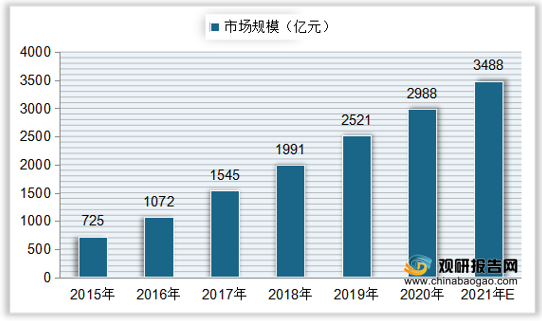
\includegraphics[scale=0.7]{494ac775492f4082a7531cfe9afdc63c.png}
\end{center}

目前我国宠物类型较多,其中猫狗类宠物较受人们的喜爱,占据我国宠物市场主导地位。据统计,2020年犬系宠物占我国宠物市场的70\%,排名第一;其次是猫系宠物,占比达到56\%;然后是水族类,占比为16\%;相对来说鸟类、爬行类和兔子类宠物占比较少,均为9\%;啮齿类与两栖类更加稀有,占比分别为6\%、4\%。

细分市场来看,在2020年我国宠物行业市场中,宠物食品类目是我国宠物行业最大的细分市场,市场分额占比达到40\%;其次是宠物医疗类,市场份额占比20\%;然后是宠物用品与宠物交易方面,占比均为10\%;水族异宠类市场份额为8\%。

\subsection{竞品分析}
根据市场调研,目前国内主流的综合宠物服务平台是波奇网、E宠商城、宠物家,他们分别属于宠物服务类的前3名。其中波奇网、E宠商城绝对是宠物服务领域的主要竞争对手。E宠商城前身是全国大型宠物门户网站——E宠网,在2009年下半年E宠商城上线,从社区转向电子商务。E宠价值观为“正品、精选、简单”,先后与海内外748家知名宠物品牌商或其代理商合作,向中国养宠家庭提供优质服务和正品保障的宠物用品。波奇网是一站式宠物综合服务网站,拥有波奇商城(线上电商)、波奇宠物服务与新零售(线下)、宠物社交(涵盖宠物社区、宠物百科等) 三大业务板块。波奇网不但涵盖了犬猫与水族等其它小宠商品品牌干粮、湿粮、零食、香波、服饰笼窝等商品,开展寄养、美容、绝育、医疗等服务。据202 财报显示,波奇宠物总营收达到10.1亿元人民币,履单后毛利提升至9.2\%,ARPU(平均用户消费金额)达到634.8 元,同比上涨33.2\%。宠物家是综合性宠物服务与商品零售品牌,成立于2015 年,现已在北京、深圳拥有近40 家直营店,拥有200 余美容师队伍,为几十万宠友提供:宠物洗美、特色服务、商品零售、寄养等高质量“平价服务”与“平价商品”。在2019 年9 月4 日,宠物家宣布完成规模近亿元的新一轮融资,由金融和房地产背景的上海鼙鼓领投,风险投资机构熊猫资本跟投。在宠物APP 方面,专营宠物相关的APP 种类丰富,但是他们并不是主要竞品,在小圈子内有所影响力但是市场规模不够庞大。

对上述主要竞品我们进行如下分析。波奇网的产品主要有客户端的网站以及移动端的波奇宠物,E宠有客户端的网站E宠商城以及移动端的E宠,与现有的在线社交购物平台淘宝京东等相似。波奇网和E 宠商城的优势都是进入宠物服务市场早,在宠物综合服务领域深耕多年,有早期积累起来的经验以及口碑优势,已经经历了多轮融资,与宠物行业上游企业建立起了稳定的合作伙伴关系。同时他们的主要业务是宠物用品电商,同时覆盖其他宠物在线服务,包含宠物社交。波奇网在移动端有宠物社区,可以有文字和视频的分享,以及本地用户的文字视频动态。E宠商城在移动端有“小宠书”,涵盖宠物在线问诊,宠物疾病知识问答,宠物主分享的视频动态以及宠物专家的知识讲堂。但是他们主营的依旧是线上电商平台,难以获取新的增长点。以波奇为例,通过其招股书显示,IPO募集资金的7000万美元资金中,波奇还是将电商作为主要的业务模式之一,这也就意味着,短时间内波奇依旧无法摆脱对第三方合作伙伴的依赖,以及无法扭转亏损的局面。同时,波奇沉淀了十多年的社区业务,从流量角度,虽然波奇社区在流量获取上起到关键作用,与传统电商的来自广告获客的模式不同,主要是基于波奇社区的内容、私域流量及泛社区来低成本获取用户。波奇宠物的广告费用主要为获客费用和品牌推广费用,2020财年总计为6900万人民币,占整体收入10\%不到,远远低于通常电商获客25\%的推广费成本。 随着私域流量开始大行其道,像公众号、微信群这些载体也正在发挥着跟波奇社区一样的作用。波奇用13年建立起来的护城河,正在受到私域流量的冲击。宠物家的优势是直营,可以把控产品服务质量的品质以及标准化操作,减少产品和服务质量的成本。但是,由于宠物家的直营模式,其拓展范围受限于养宠程度密集且对于服务质量和需求大的一二线城市,例如北京、深圳等,如果继续渗透中小城市,对其供应链、人员培训以及管理模式会带来更加巨大的挑战。但是宠物市场下沉趋势明显,宠物家的模式有着一定的缺陷。

\begin{center}
  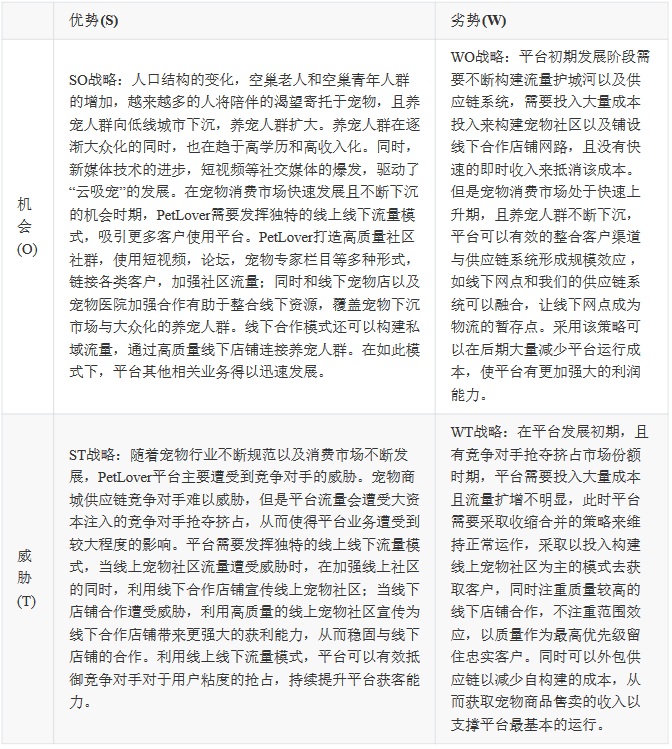
\includegraphics[scale=0.7]{QQ截图20220114220853.png}
\end{center}

\section{主要产品介绍}

\subsection{产品描述}
为了满足目标客户群体的需求,为宠物爱好者真正提供一个一站式综合服务宠物平台,PetLover平台主要提供三大功能模块:宠物商城、宠物社区、宠物医疗及宠物百科。其中宠物商城主要提供宠物购买、宠物用品购买及宠物服务购买等服务,为用户提供商品质量保证,并以完善的供应链渠道为用户提供良好的购物体验;宠物社区则为宠物爱好者、动物保护志愿者提供了一个宠物饲养交流、宠物知识分享及动物保护理念宣传的社区平台,在社区中,用户共同创造价值,产出高质量的知识性资源,共同维护爱宠社区健康发展;宠物百科则通过引入宠物专家分享的宠物知识及社区中高质量宠物知识/经验分享帖相关内容,对养宠知识进行整合分类,方便用户进行指定知识的查阅;宠物医疗服务则通过以兼职平台的形式引入专业宠物医师、专家等,为养宠用户提供专业的宠物护理及诊疗建议,并与线下宠物医院等开展合作、建立线下宠物诊疗网点。

\subsection{功能介绍}
\begin{itemize}
  \item \textbf{宠物商城}:平台提供宠物商城服务,包括宠物购买、宠物用品购买及宠物服务购买等服务,为用户提供商品质量保证,并以完善的供应链渠道为用户提供良好的购物体验。具体来讲,应该包括如下细节功能:
  \begin{itemize}
    \item \textbf{查看商品}:用户可以进入商品详情页,对商品的细节、参数、适用范围等内容进行查阅
    \item \textbf{查看商品测评}:用户可以查看欲购买商品的相关测评/种草秀,以帮助选购商品
    \item \textbf{查看商品评价}:用户可以查看某一商品的其他用户评价,通过好评率、评价内容等指标帮助选购商品
    \item \textbf{购买商品}:用户选定商品后,可以购买该商品,并可以设置商品数量、商品小类、付款方式、送货时间、收货地址等
    \item \textbf{评价商品}:用户购买商品后,可以选择对商品进行评价,以帮助其他用户选购
    \item \textbf{测评商品}:用户购买商品后,可以选择对商品进行测评并发布测评/种草秀等,以帮助其他用户选购
    \item \textbf{添加/修改商品信息}:对于商品供应商,他们可以添加商品或修改某一商品的信息(如价格、规格、小类等)
  \end{itemize}
  \item \textbf{宠物社区}:平台提供宠物社区功能,这是一个宠物饲养交流、宠物知识分享及动物保护理念宣传的社区平台。具体来讲,应该包括如下细节功能:
  \begin{itemize}
    \item \textbf{按话题查看社区帖子}:用户可以根据自身需求按话题进入不同社区的版块,并查看对应版块中的帖子
    \item \textbf{搜索社区帖子}:用户可以在社区中进行全社区搜索,或在某一版块主题下搜索相应的帖子
    \item \textbf{回帖}:用户可以在某一帖子下发表回复,也可以在某一层回复下进行回复
    \item \textbf{发帖}:用户可以在某一社区版块主题中进行发帖
    \item \textbf{消息通知}:当用户的帖子被回复或用户在其他帖子中的回复被回复时,用户可以收到相应的消息通知
    \item \textbf{举报}:用户可对社区中某些帖子进行举报,举报后交由社区管理员进行审核
    \item \textbf{删帖}:用户可以删除自己发布的帖子;社区管理员可以删除普通用户的发帖
    \item \textbf{删除回复}:用户可以删除自己的某条回复
    \item \textbf{精华帖}:用户可以申请将自己的帖子设为精华帖;社区管理员可以审核用户申请,并将某一用户帖设置为精华帖
    \item \textbf{百科帖}:社区管理员可以对精华帖进行审核筛选,并将较为专业和优质的帖子设置为百科帖,允许用户在宠物百科中查看这些百科帖
  \end{itemize}
  \item \textbf{宠物百科}:平台提供宠物百科服务,通过引入宠物专家分享的宠物知识及社区中高质量宠物知识/经验分享帖相关内容,对养宠知识进行整合分类,方便用户进行指定知识的查阅。具体来讲,应该包括如下细节功能:
  \begin{itemize}
    \item \textbf{查看宠物百科}:用户可以进入宠物百科并查看某篇百科内容
    \item \textbf{审核宠物百科}:平台管理员可以对宠物百科内容进行审核
    \item \textbf{编辑宠物百科}:平台管理员或百科创作者可以对宠物百科内容进行编辑,编辑后需再交由平台管理员审核,审核通过后方可显示编辑后的内容
    \item \textbf{点赞}:用户可对宠物百科内容进行点赞
    \item \textbf{内容求助}:若宠物百科中没有用户需要的内容,用户可发起内容求助,即向平台提交针对某一特定的、宠物百科中尚不存在的内容的申请,申请交由平台管理员进行审核
    \item \textbf{内容勘误}:若宠物百科中出现了错漏之处,用户可发起内容勘误,即向平台提交针对某一特定宠物百科内容中的错漏之处的更改申请,申请交由平台管理员进行审核
  \end{itemize}
  \item \textbf{宠物医疗}:平台提供宠物医疗服务,通过以兼职平台的形式引入专业宠物医师、专家等,为养宠用户提供专业的宠物护理及诊疗建议。具体来讲,应当包括如下细节功能:
  \begin{itemize}
    \item \textbf{查看宠物护理建议}:用户可以在宠物医疗服务版块浏览来自专业宠物医师的宠物护理建议,如疾病预防建议、宠物膳食管理、宠物习惯培养等
    \item \textbf{查看宠物疾病常识}:用户可以在宠物医疗服务版块浏览来自专业宠物医师的宠物疾病知识,以了解宠物常见疾病、预防方式、应对措施等
    \item \textbf{查看宠物医师列表}:用户可以在宠物医疗服务版块浏览常驻PetLover平台的宠物医师列表,查看医师的基本信息(如资历、医师评价、擅长领域、工作地点等),以帮助用户选择咨询的医师
    \item \textbf{预约诊疗}:用户可以在宠物医疗服务版块中向某医师进行诊疗预约,预约时,用户需指明问诊时间(如立即、一天后、两天后)、宠物类型、疾病类型等
    \item \textbf{接受诊疗预约}:物医师在接到来自用户的诊疗预约后,可以选择接受或拒绝诊疗预约
    \item \textbf{宠物问诊}:养宠用户和宠物医师可以在预约的时间以线上对话或电话的形式进行宠物问诊,在进行线上对话时,用户可以发送图片和文字,医师可以发送语音和文字
    \item \textbf{用药推荐}:宠物医师可根据养宠用户描述的病情为其推荐宠物用药,并在对话框中进行显示
    \item \textbf{病情跟踪}:养宠用户在进行完一次问诊后,可以选择是否开通病情跟踪功能,开启后,用户可以在限定的时间内再次对相同医师发起免费问诊服务,系统也将保留用户和该医师的历史对话记录
    \item \textbf{线下问诊预约}:用户可以选择当地宠物诊疗的线下网点进行线下问诊预约,预约时需指定网点名和前往时间
    \item \textbf{医师评价}:在进行一次宠物问诊后,用户可以对医师进行评价,包括专业度、满意度等指标
    \item \textbf{宠物医疗网点评价}:在进行一次线下问诊后,用户可以对线下问诊所在的医疗网点进行评价,包括专业度、满意度、服务态度等指标
  \end{itemize}
\end{itemize}

\subsection{使用场景}

\subsubsection{宠物爱好者}
\begin{itemize}
  \item 场景IP:想宠就“宠”,不再“云吸宠”;说出你的养宠趣事
  \item 场景分发:“云吸宠”(看宠物小视频时)对养宠物的心动,通过有保障的养宠攻略以及快捷有保障获得宠物的方式,让心动者行动。同时,捕获养宠人社交心态,放大分享动机推进分享养宠趣事。
  \item 了解并评估:晓琳在搜索养猫攻略时,发现了这个平台。但是一开始她以为这只是一个宠物用品商城,就草草地略过了。晓琳在“云吸猫”时发现了一个优质的宠物博主在PetLover平台上也有分享,就对平台进行了一番细致了探索。晓琳发现了平台其他宠物爱好者详细地养宠经历与趣味小视频,更有养宠经验与忠告,加之有知名宠物博主的入驻,晓琳对PetLover平台上的养宠经验可靠性充满了信心。
  \item 购买并传递获得:晓琳购买心仪品种的小猫是在PetLover的宠物交易模块进行,她通过了模块何附近的宠物店进行了线上联系与咨询,但是并没有找到。在浏览附近其他地区的宠物商店时,发现了宠物竟然可以快递邮寄,而且有专门的保障服务。这让晓琳欣喜狂,同时根据攻略在宠物用品模块购买了相应的宠物用品。当小猫健康平安地送达,蜷缩在笼子里时,晓琳悬着的心也放了下来。
  \item 交互:当遇到宠物问题时,晓琳继续查看PetLover上的养宠攻略,获取进一步的建议;悠闲时刻,晓琳也会看看其他人的养宠趣闻,惹得晓琳忍俊不禁;晓琳也会刷刷宠物商城,看看有没有想要的给小猫添置的宠物用品,宠物食品。
  \item 售后:晓琳很担心宠物的邮寄问题,但是平台的快递承诺——保证宠物安全送达,不然由平台承担费用损失,让晓琳稍微放心了下来。晓琳对某件宠物用品在不太满意,平台允许7天无理由退换的要求满足了晓琳这样的有充分购买欲望但是不知道商品用处是否很大的宠物爱好者。
  \item 评价与复购:晓琳对平台很满意,能够在平台满足自己全方位的养宠需求。晓琳认为平台值得继续使用。
\end{itemize}

\subsubsection{宠物医疗行业从事者}
\begin{itemize}
  \item 场景IP:你值得更大的舞台。
  \item 场景分发:对于N线小城市的从事宠物医疗服务人员,由于地理原因处于小城市,无法充分发挥自己的专业知识,创造更多的价值。宠物在线咨询给他们提供了更大的平台发挥自己的专业知识价值。
  \item 了解并评估:阿添在所在的宠物医院和PetLover平台合作是了解到这个平台。入驻后,发现这个平台的客流量很高,同时可以通过空闲时间回答问题给出专业建议而获得一定地兼职收入,这让阿添的目标——给更多地宠物看病从而获得更高地收入,得以实现。
  \item 购买并传递获得:阿添入驻PetLover咨询医师,在每回答一个问题之后,都会得到平台的收入补贴。
  \item 交互:PetLover平台会推荐问题给每个入驻咨询医师。阿添可以从中选择自己擅长的问题来回答。在每次回答完后,都会有相应的评价回复提示,这让阿添能够得到及时的反馈。
  \item 售后:阿添在某次回答了问题却没有收到平台提供的补贴,这让阿添有点愤怒。阿添发现平台提供了申诉模块,赶忙去申诉。平台在5分钟左右就回复了阿添的申诉,很快就把补贴发送到了阿添的账户上,并且给了阿添额外的补贴作为赔偿,这让阿添心里的火气降了下来。
  \item 评价与复购:阿添对平台庞大的流量以及能够通过发挥自己的专业知识来得到额外的报酬十分满意,在空闲时间会持续使用平台。
\end{itemize}
\subsubsection{宠物及用品供应商}
\begin{itemize}
  \item 场景IP:解决电商“最后一公里“问题;线下店铺线上宣传。
  \item 场景分发:对于有志于拓展线上业务的宠物用品店,需要额外的人力来专注于快递的发送,无疑增加了开线上店铺的成本。平台通过解决快递这样的”最后一公里“问题,让店铺专注产品质量;线下店铺可以通过线上宣传增加知名度。
  \item 了解并评估:小川的一个养宠朋友给他推荐了PetLover平台。小川得知平台上面入驻了不少宠物用品商店,但是他们所在城市并没有宠物用品店的线下网点,于是果断联系PetLover平台入驻。
  \item 购买并传递获得:小川所经营的宠物用品商店成为了当地第一家PetLover的线下网点,同时在平台的帮助下解决了没有额外人力参与邮寄商品的问题,平台会负责商品的邮寄,小川只需要把商品打包即可,因此小川的网店也在平台上重新开始经营。由于平台的流量,小川的线下商店知名度也越来越高,吸引很多当地的PetLover用户来购买。
  \item 交互:平台在每个订单到来时,小川会收到提示按照约定的时间将商品列表打好包,让平台来负责邮寄。同时用户对于商店评价也会及时给小川反馈。
  \item 售后:无(可以按照意愿,随时退出平台)
  \item 评价与复购:在平台流量的加持,以及平台快递支撑下,小川的店铺越做越好,小川对于入驻平台十分满意,希望能够在平台上面越做越大。
\end{itemize}
\subsubsection{动物保护志愿者}
\begin{itemize}
  \item 场景IP:你的行动应该被看见。
  \item 场景分发:对于有志于保护小动物的动物保护志愿者,苦于传统宣传手段的局限性,受众对象和传播广度受限,没有办法充分宣传保护流浪动物的精神,让更多愿意加入保护流浪动物的有志者。利用流量优势让动物保护志愿者的行动与声音被更多地宠物爱好者知道,让动物保护志愿者的理想得到满足。
  \item 了解并评估:淑元了解到中国小动物保护协会与PetLover进行了合作,获得了中国小动物保护协会的授权。中国小动物保护协会的认可给予了淑元信心,淑元随即就注册了一个账号,希望能够让自己的理念被更多人了解并传播。
  \item 购买并传递获得:淑元以志愿者的身份,发布了一些关于当地小动物保护的推文,很快就获得了许多宠物爱好者和宠物店主,咨询医师等人的关注。当地的宠物医院与流浪猫救助协会联系上了淑元,邀请她一同参与正在进行的小动物救助的项目。这让淑元十分开心。
  \item 交互:当淑元的推文发出去之后,都会获得一系列回复的提示,都是对淑元的鼓励。这让淑元更加充满动力。
  \item 售后:无
  \item 评价与复购:淑元觉得平台是自己宣传保护小动物精神的广阔窗口,在这里进行宣传比起自己一个人面对面的宣传,有着受众面更加有效与传播面更加广泛的优势。淑元认为自己会把自己的行动放在平台上,持续利用线上线下结合的方式,更好地宣传保护小动物的精神。
\end{itemize}

\section{财务分析}

\subsection{投融资分析}

\subsubsection{股本结构与规模}

本项目预计注册资本200万,其中创业团队将出资80万,南京大学双创中心提供资金为20万,面向社会引资60万,长期贷款40万;项目投入运营后希望引入200万天使投资作为流动资金。

由于成本结构的限制以及技术的要求,PetLover项目前期投入较高,前期投入全部利用经费解决。初始投资将用于社区搭建与维护、宣传吸引宠物及其用品商家、与宠物医疗部门和人员、知识分享博主等合作、云服务器等实物资源购买与维护,初期投入(第一年)资金分配预测如下表:

\newpage

% Please add the following required packages to your document preamble:
% \usepackage[table,xcdraw]{xcolor}
% If you use beamer only pass "xcolor=table" option, i.e. \documentclass[xcolor=table]{beamer}
\begin{table}[]\centering
  \begin{tabular}{|
  >{\columncolor[HTML]{FFFFFF}}c |
  >{\columncolor[HTML]{FFFFFF}}c |
  >{\columncolor[HTML]{FFFFFF}}c |
  >{\columncolor[HTML]{FFFFFF}}c |
  >{\columncolor[HTML]{FFFFFF}}c |
  >{\columncolor[HTML]{FFFFFF}}c |
  >{\columncolor[HTML]{FFFFFF}}l |}
  \hline
  前期投入资金分配(单位:万元) & 员工工资 & 设备成本 & 广告成本 & 合作成本 & 其他 & 合计  \\ \hline
  资金              & 20   & 10   & 40   & 100   & 30 & 200 \\ \hline
  \end{tabular}
  \end{table}

  同时,为了减少财务杠杆为初创企业带来的财务风险与偿债压力,也为了利用天使投资在相关行业的企业矩阵资源,团队决定利用股权融资而非债权融资,创始团队拥有87.5\%的要求权,保证创始团队对项目的控制权与项目运行的稳定性。
  
  \subsubsection{投资收益分析}

  中国宠物市场,典型的蓝海领域。不管是一级市场,还是二级市场均纷纷看好,不管是美国,还是中国均是如此。

  在一级市场中,2018年国内宠物行业发生融资案例30多起,融资额超过15亿元,包括高瓴、纪源、IDG等知名投资机构先后入场。2019年,融资事件更是达到41起,累计吸金规模超过42亿元。在这个赛道,高瓴尤其是重仓看好,在2016-2018年三年中斥资至少10亿美元,投了100多家宠物企业,包括芭比堂、宠物家、爱诺、龟与熊猫、瑞鹏集团等品牌。

  在二级市场,美国纯玩宠物电子零售商Chewy于2019年6月挂牌交易日,到2020年12月已经累计上涨超过410\%,当前最新市值已经高达446亿美元。另外,宠物服务商PetSmart很早就登陆资本市场,股价长期上涨,后于2015年被私有化了,上市期间最大的涨幅为4000\%。

  在中国,中宠股份于2017年8月登陆创业板,主营为宠物食品。截止至2020年12月,中宠已经累计上涨560\%,,短短3年半时间就取得如此巨大的涨幅。

  据《2019年中国宠物行业白皮书》显示,2010-2019年,中国城镇宠物行业市场规模逐年提升,年复合增速达到34.55\%。至2019年,中国养宠家庭数量为9978万户,市场规模突破2000亿大关,同比增长近20\%。预计到2024年,市场规模将达到4500亿元左右,年复合增速仍然高达17.3\%。

  宠物行业增速如此之快,蛋糕越来越大,孕育的投资机会不少,自然会有资本趋之如骛,投资形势一片大好。

\subsection{财务预测}

PetLover项目围绕建立宠物社区平台为核心,为宠物市场提供宠物商品买卖、宠物医疗服务、宠物知识问答、宠物日常分享等服务,同时会在线下设置服务网点,辐射一片区域的用户,为他们提供宠物上门服务。

PetLover的主要成本有员工工资、设备成本、广告成本、合作成本。软件在开发阶段需要有开发人员持续进行开发,软件发布之后需要有客服人员以及维护人员持续提供服务,这些开发与维护人员的薪资均属于不可变的固定成本;在软件开发初期,一般使用成型的云服务平台,需要支付云服务器的费用。在办公室中还需要支付一定的费用对职员的办公设备进行购买与维护;在软件宣传的过程中,需要大量的广告宣传来提高知名度,扩充基础个人用户量,维持日活跃用户流量,因此需要提供适当的广告营销成本进行推广;为了让平台拥有初始的精品笔记分享、常驻的宠物医师以及宠物店,来打造平台的原生社区环境,还需要支付聘请宠物博主、宠物医师以及加盟宠物店的合作费。

PetLover的收入来源有自营产品销售、平台费用、广告费。平台支持宠物以及宠物用品交易,提供自营店与专卖店,掌握供应链,完善售后客服,提供一系列完整的消费服务,从中收取资产销售费用;为了方便用户接受线下品牌实体店的服务,平台支持第三方宠物店交易以及宠物医院问诊,在服务过程中提供支付平台,从中收取交易手续费;平台还提供一些区域作为发布广告的场所(规定投放广告的质量以及出现频率要求,以为普通用户提供优质的使用体验为最终目的),从广告厂商处收取费用。

PetLover平台力求投入第一年即获得高收益,投入运营的第一年至第五年资产预测表如下:

\newpage
% Please add the following required packages to your document preamble:
% \usepackage[table,xcdraw]{xcolor}
% If you use beamer only pass "xcolor=table" option, i.e. \documentclass[xcolor=table]{beamer}
\begin{table}[]\centering
  \begin{tabular}{|
  >{\columncolor[HTML]{FFFFFF}}c |
  >{\columncolor[HTML]{FFFFFF}}c |
  >{\columncolor[HTML]{FFFFFF}}c |
  >{\columncolor[HTML]{FFFFFF}}c |
  >{\columncolor[HTML]{FFFFFF}}c |
  >{\columncolor[HTML]{FFFFFF}}c |
  >{\columncolor[HTML]{FFFFFF}}c |}
  \hline
  资产(单位:万元) & 初期  & 第一年末 & 第二年末 & 第三年末 & 第四年末 & 第五年末 \\ \hline
  现金        & 200 & 185  & 317  & 492  & 749  & 1136 \\ \hline
  短期投资      & —   & —    & —    & —    & —    & —    \\ \hline
  预付款项      & —   & 194  & 322  & 500  & 745  & 1010 \\ \hline
  存货        & —   & 6    & 6    & 17   & 20   & 28   \\ \hline
  待摊费用      & —   & —    & —    & 6    & 10   & 14   \\ \hline
  流动资产      & 200 & 385  & 645  & 1015 & 1514 & 2188 \\ \hline
  固定资产总额    & —   & 40   & 32   & 42   & 67   & 84   \\ \hline
  累计折旧      & —   & 8    & 6    & 8    & 14   & 20   \\ \hline
  固定资产净值    & —   & 32   & 25   & 35   & 52   & 62   \\ \hline
  无形资产      & —   & 24   & 40   & 64   & 45   & 116  \\ \hline
  资产合计      & 200 & 441  & 710  & 1114 & 1611 & 2366 \\ \hline
  \end{tabular}
  \end{table}

  PetLover平台的投入运营的第一年至第五年负债和所有者权益预测表如下:

  \newpage
% Please add the following required packages to your document preamble:
% \usepackage[table,xcdraw]{xcolor}
% If you use beamer only pass "xcolor=table" option, i.e. \documentclass[xcolor=table]{beamer}
\begin{table}[]\centering
  \begin{tabular}{|
  >{\columncolor[HTML]{FFFFFF}}c |
  >{\columncolor[HTML]{FFFFFF}}c |
  >{\columncolor[HTML]{FFFFFF}}c |
  >{\columncolor[HTML]{FFFFFF}}c |
  >{\columncolor[HTML]{FFFFFF}}c |
  >{\columncolor[HTML]{FFFFFF}}c |
  >{\columncolor[HTML]{FFFFFF}}c |}
  \hline
  负债和所有者权益(单位:万元) & 初期  & 第一年末 & 第二年末 & 第三年末 & 第四年末 & 第五年末 \\ \hline
  短期借款            & —   & —    & —    & —    & —    & —    \\ \hline
  应付工资            & —   & 64   & 64   & 96   & 112  & 120  \\ \hline
  应付税金            & —   & 66   & 186  & 355  & 438  & 556  \\ \hline
  其他应付款           & —   & 48   & 40   & 48   & 140  & 209  \\ \hline
  流动负债合计          & —   & 180  & 290  & 500  & 690  & 885  \\ \hline
  长期负债            & 40  & 52   & 53   & 0    & 0    & 0    \\ \hline
  实收资本            & 160 & 160  & 160  & 160  & 160  & 160  \\ \hline
  资本公积            & —   & —    & —    & —    & —    & —    \\ \hline
  盈余公积            & —   & 10   & 28   & 54   & 66   & 84   \\ \hline
  未分配利润           & —   & 41   & 180  & 328  & 741  & 1240 \\ \hline
  负债和所有者权益合计      & 200 & 443  & 711  & 1042 & 1657 & 2369 \\ \hline
  \end{tabular}
  \end{table}

  PetLover平台的投入运营的第一年至第五年收益预测表如下:

  \newpage
% Please add the following required packages to your document preamble:
% \usepackage[table,xcdraw]{xcolor}
% If you use beamer only pass "xcolor=table" option, i.e. \documentclass[xcolor=table]{beamer}
\begin{table}[]\centering
  \begin{tabular}{|
  >{\columncolor[HTML]{FFFFFF}}c |
  >{\columncolor[HTML]{FFFFFF}}c |
  >{\columncolor[HTML]{FFFFFF}}c |
  >{\columncolor[HTML]{FFFFFF}}c |
  >{\columncolor[HTML]{FFFFFF}}c |
  >{\columncolor[HTML]{FFFFFF}}c |}
  \hline
  收益(单位:万元)    & 第一年 & 第二年 & 第三年 & 第四年  & 第五年  \\ \hline
  一、主营业务收入     & 328 & 600 & 880 & 1120 & 1440 \\ \hline
  减:主营业务成本     & 75  & 85  & 92  & 122  & 136  \\ \hline
  减:主营业务税金即附加  & 16  & 16  & 22  & 24   & 27   \\ \hline
  二、主营业务利润(毛利) & 237 & 499 & 766 & 974  & 1277 \\ \hline
  加:其他业务利润     & 15  & 17  & 25  & 30   & 38   \\ \hline
  减:营业费用       & 64  & 18  & 22  & 25   & 28   \\ \hline
  减:管理费用       & 2   & 2   & 5   & 7    & 9    \\ \hline
  减:财务费用       & 3   & 2   & 2   & 3    & 5    \\ \hline
  三、营业利润       & 183 & 494 & 762 & 969  & 1273 \\ \hline
  加:投资收益       & 0   & 0   & 180 & 180  & 182  \\ \hline
  加:营业外收入      & 0   & 0   & 10  & 24   & 30   \\ \hline
  减:营业外支出      & 16  & 26  & 62  & 77   & 94   \\ \hline
  减:所得税费用      & 67  & 187 & 356 & 438  & 556  \\ \hline
  四、净利润        & 100 & 281 & 534 & 658  & 835  \\ \hline
  \end{tabular}
  \end{table}
\subsection{财务比率分析}
为了对公司的财务状况进行客观分析和评价,从而为投资者、经营者及其他利益相关者提供了解公司过去,评价现状,预测公司未来发展的信息,现对公司的偿债能力、营运能力及盈利能力等进行分析,我们分别选取了它们的相关指标,分析如下:

\subsubsection{偿债能力}
债务是企业在未来要偿还的以前经济业务所承担的经济责任,偿债能力关系到筹资活动的风险,公司如不能按期足额偿付债务,则会面临一系列损失。下面从流动比率\footnote{流动比率是流动资产对流动负债的比率,用来衡量企业流动资产在短期债务到期以前,可以变为现金用于偿还负债的能力。一般认为流动比率在2左右比较好,表明公司有较好的短期债偿还能力。}、速动比率\footnote{速动比率是速动资产对流动负债的比率,用来衡量企业流动资产中可以立即变现用于偿还流动负债的能力。一般认为维持在1左右比较好,表明公司短期偿债能力有可靠的保证。}两方面进行分析:

\newpage
\begin{table}[]\centering
  \begin{tabular}{llllll}
       & 第一年 & 第二年 & 第三年 & 第四年 & 第五年 \\
  流动比率 & 2.14 & 2.22 & 2.03 & 2.19 & 2.47 \\
  速动比率 & 1.03 & 1.09 & 0.98 & 1.08 & 1.28
  \end{tabular}
  \end{table}

  \subsubsection{营运能力}
  营运能力能反应公司对有限资源的配置和利用能力,为了反应公司的营运能力,从流动资产周转率\footnote{流动资产周转率指企业一定时期内主营业务收取净额同平均流动资产总额的比率,是评价企业资产利用率的重要指标,一般认为流动资产周转率大于2时,企业资产利用率较高。}进行分析。

  \newpage
  \begin{table}[]\centering
    \begin{tabular}{llllll}
            & 第一年  & 第二年  & 第三年  & 第四年  & 第五年  \\
    流动资产周转率 & 0.852 & 0.930 & 0.867 & 0.740 & 0.858
    \end{tabular}
    \end{table}

    \subsubsection{盈利能力}
    盈利能力是公司在一定时期内赚取利润的动力,反映了公司成本费用管理的效果问题,为了反映公司的盈利能力,从净资产收益率\footnote{净资产收益率是净利润与平均股东权益的百分比,是公司税后利润除以净资产得到的百分比率,反映股东权益的收益水平,可以衡量公司运用自有资本的效率,指标越高,说明自有资本获得净收益的能力越强。}进行分析。
    
    \newpage
    \begin{table}[]\centering
      \begin{tabular}{llllll}
             & 第一年   & 第二年   & 第三年   & 第四年   & 第五年   \\
      净资产收益率 & 22.7\% & 39.6\% & 47.9\% & 40.8\% & 35.3\%
      \end{tabular}
      \end{table}

      通过以上对本公司的偿债能力、营运能力及盈利能力的分析,可以看到,公司偿债能力较强,能很轻松地偿还当年的短期贷款;公司流动资产周转率比较低,企业资产利用率就比较低,运营能力不足;公司的资产收益率高,投资回报率高且增长较快,可见公司的盈利能力较强,公司投资方案可行。
      
\section{运营规划}

\subsection{产品开发规划}
开发规划时间节点相对于项目启动时间展开,具体开发规划如下:

\begin{itemize}
  \item 在项目启动一个月内,完成对PetLover平台的需求获取工作,该阶段需要投入资金吸引需求获取对象,包括宠物爱好者、宠物商品卖家、宠物医疗行业从事者、中午知识分享博主等。
  \item 在项目启动第一个月后到第二个月,完成对需求获取阶段的整理和过个说明,力求对PetLover平台需求的严格说明,尽可能减少后续其软件开发过程中的需求变更。
  \item 在项目启动的第三个月上旬,完成PetLover平台开发的具体分工,包括前后端开发、服务器部署和管理、测试工作、需求变更工作等。
  \item 在项目启动的第三个月和第四个月,完成PetLover平台的第一轮迭代,功能覆盖主营业务,包括宠物社区、宠物商城、宠物医疗咨询和服务,并进行功能集成测试。
  \item 在项目启动的第五个月,面向用户进行测试。
  \item 在项目启动的第六个月,PetLover平台迭代一正式发布,其实现功能覆盖主营业务。
  \item 项目启动第六个月后,PetLover平台运营迭代双线程,逐步实现增值服务和未来产品布局所描述的服务。
\end{itemize}

\subsection{市场策略及业务拓展计划}
PetLover作为一款专注于为养宠者提供一站式综合服务的产品,需要对受众客户进行较好的定位,因此可以从微博、小红书、B站、抖音等平台针对知名的宠物类博主进行软广告投放,帮助我们精准定位会对产品感兴趣的受众人群。同时在上述平台进行造势活动,借助KOL进行平台推广,发挥KOL的粉丝黏性。

\subsubsection{市场推广策略}
\paragraph{第一阶段:小范围测试推广}奠定产品的平台开发基础,以及系统运行前期试验阶段的双向资源,收集整合多方面信息完善平台开发,进一步深入市场探求深度潜在需求。同时在大流量平台举办造势活动,积累下产品的原始用户。
\paragraph{第二阶段:SNS营销}建立微信公众号、微博认证号等各平台公共主页,通过定期内容输出、活动举办达到引流目的。在微博、小红书、B站等平台进行一定规模的广告投放。在这一阶段,需要着重提高产品日活跃用户量。
\paragraph{第三阶段:链式传播、社区运营}这一阶段主要提高用户粘性并增加其分享次数,以达到产品的链式传播。同时开始进行产品社群运营,打造自己的KOL,逐渐降低产品的CPM。

\subsubsection{市场品牌策略}
PetLover致力于解决养宠用户:养宠点滴无法分享、养宠知识难以获取、宠物生病手忙脚乱等痛点,提供高质量宠物社区社群,推荐养宠干货,分享养宠心得,并且与线下网点合作为大多数普通养宠用户提供平价质量有保障的宠物用品与宠物服务。

\subsubsection{市场渠道策略}
\paragraph{起步阶段:}构建相对完备的宠物用品供应链系统,同时联系各大流量平台如小红书、抖音、B站等的主要高知名度宠物博主进行产品推荐分享。
\paragraph{中间阶段:}完善宠物用品供应链系统。在投放软广告分享APP产品的基础上,和相关平台(小红书、抖音、B站等)主动联系,寻求更大的广告版位进行广告投放;同时开始线下网点的铺设,以优惠策略邀请线下宠物网点加入平台。
\paragraph{成型阶段:}这一阶段下已经拥有稳定且持续增长的日活跃用户量,线下宠物网点也处于长期合作状态,此时利用广泛的线下网点进一步宣传APP,以实现覆盖下沉市场养宠客户,形成线上线下渠道融合的状态。

\subsubsection{业务拓展规划}
\begin{itemize}
  \item 一、为宠物商城板块构建宠物用品供应链系统,为自营或加盟宠物用品商店做准备;宠物社区和宠物百科上线。
  \item 二、线下网点服务业务上线,和各地线下宠物店以及宠物医院联系合作,加入平台为用户提供预约线下服务。同时邀请优质线下网点加入宠物商城。
  \item 三、在线宠物问诊业务上线,和宠物医院中的医生合作,为养宠用户提供付费咨询服务。
  \item 四、宠物社区拓展,提供短视频分享、宠物专家养宠知识专栏等细分内容。
\end{itemize}

\subsection{财务规划}
根据财务预测,PetLover平台的投入运营的第一年至第五年收益规划如下:
\begin{itemize}
  \item 在投入运营的第一年,主营业务收入达到328万元,净利润达到100万元。
  \item 在投入运营的第二年,主营业务收入达到600万元,净利润达到281万元。
  \item 在投入运营的第三年,主营业务收入达到880万元,净利润达到534万元。
  \item 在投入运营的第四年,主营业务收入达到1120万元,净利润达到658万元。
  \item 在投入运营的第五年,主营业务收入达到1440万元,净利润达到835万元。
\end{itemize}

\subsection{团队管理}
同舟才能共济,合作才能共赢,产品的健康发展离不开团队的共同努力,拥有一个优良精干的团队,才能为完成团队目标打下良好基础。团队管理应以五大重要因素为起点:
\paragraph{目标管理:}浑浑噩噩的团队没有战斗力,疲于奔命的团队也不可能有效爆发,因此需要在团队成立之初就为团队树立一个明确可达的目标。一个清晰的目标对于整个团队都起着重要作用,我们团队必须确立“专注于宠物爱好者一站式综合平台服务”的共识,并在产品开发的过程中始终贯彻动物保护的理念,不忘初心,真正做好为宠物爱好者等目标群体打造的爱宠平台。只有在统一目标管理的作用下,团队成员共享目标,有了明确方向,才能携手共进、创造成绩。
\paragraph{有效沟通:}每个人的心态都是不同的,在出现分歧的时刻,若不及时沟通,则矛盾和隔阂会越积越深,不仅影响日常工作交流,更会在日后某一时间点爆发,而造成不可挽回的错失。团队管理必须从人的需求出发,进行有效的沟通交流,才能更好理解团队成员的真情实感、得到他们最真实的反馈,只有通过沟通完成成员情感的梳理、目标的明确,才能提升项目完成的效率。
\paragraph{流程化管理:}一个优秀的团队离不开高效的流程化管理,不以规矩、不成方圆,规划来源于整体目标的设定和拆解,当对整体目标进行拆解后,就可以指定完整的流程来一一攻克这些拆分的小目标,从而阶段性地进行团队工作的开展,进而实现团队流程化管理。如果不进行目标拆解、不进行团队流程化管理,整个团队便会如一盘散沙,团队内部不团结,更无需谈及实现一款完善的产品。
\paragraph{绩效管理:}作为团队领导者,需要对团队成员适度表达欣赏。当团队成员出色地完成了一个项目时,掌声与鼓励丝毫不能吝啬:人人都喜欢被夸赞和获得肯定,同时也要保障其能获得与付出相吻合的薪资报酬。绩效评估、津贴、奖励等都有助于激励团队成员努力工作、表现更佳。进行团队管理时需要制定一套合理、公平公正的奖励体系,这样才能激励团队成员提高工作效率、乐意为团队付出,早日实现工作目标。
\paragraph{成员关系管理:}管理团队时,亦需要对成员有一定程度的了解:他们的工作情况、擅长领域、性格特点等都需要了解清楚。创建团队很容易,但将不同性格、不同特点的团队成员绑定在一起进行团队性工作则是一件困难的事。团队领导者需要加强管理团队成员之间的关系,创造一个他们之间可以相互信任的环境,首先要避免团队内部拉帮结伙,然后也要重视团队领导者和团队成员之间的良好关系:团队的本质不是单打独斗,而是同舟共济

\section{风险预测及解决方案}

\subsection{风险识别}

\subsubsection{市场推广风险}
\begin{itemize}
  \item 对宠物行业预测不准确:虽然近几年的宠物市场在不断扩张,但由于受疫情影响,人们的平均收入减少,人们的消费水平和消费观念可能受到影响,对宠物饲养的投入可能会减少。因此未来几年的宠物行业仍然不容乐观,如果宠物市场在近几年萎缩,PetLover平台将会入不敷出,最终销声匿迹
  \item 宠物行业主流玩家(大型平台)带来竞争压力:作为学生团队,我们波奇网、E宠商城等大型宠物平台相比,必然会出现资金有限、缺少大量数据的支撑、技术不够完备、没有知名度等等一系列问题,这将会使我们在竞争中处于劣势。
\end{itemize}
\subsubsection{技术风险}
\begin{itemize}
  \item 技术建议,容易替代:由于PetLover技术方面要求并不高,如果市场方面没有到位,很容易会被新进入的类似产品替代,如果我们在后期没有继续更新自己的服务、完善应用的功能、推出新的卖点,后期进入的潜在对手能够提供我们产品大部分的功能,可能会在规模、价格上使我们陷入困境。
  \item 服务质量无法达到预期:由于PetLover团队初期规模小,技术等不完善,力量有限,当用户不再满足于现有的服务,在产品的技术层面提出更高的要求时,我们可能无法快速高质量地进行反馈。
\end{itemize}
\subsubsection{法律道德风险}
\begin{itemize}
  \item 市场垄断风险:大型宠物平台可能通过市场扩张、压低费用等方式抢占新进入宠物市场者的市场,新进入市场者可能举步维艰。
  \item 隐私泄露风险:PetLover平台掌握平台用户的用户信息、合作商家的商品信息、合作医疗机构或人员的隐私信息,这些信息可能会通过公司内外不明交易泄漏到外界,侵犯用户隐私没产生隐私泄露纠纷,损害公司名誉。
  \item 合同风险:由于我们的团队缺少企业经营经验,在交易活动中可能会出现合同风险,尤其是与其他市场主体签订合同时因存在问题而产生纠纷。包括因合同主体存在问题而产生的纠纷,合同条款不完善而导致的纠纷,合同履行过程中产生的纠纷等。
\end{itemize}
\subsubsection{财务风险}
\begin{itemize}
  \item 资金无法回收:PetLover项目在前期需要少量资金投入启动,但是由于不稳定因素及知名度低等劣势,前期的投入可能无法获得收益,甚至难以回收成本。
  \item 资金融通风险:随着PetLover平台的发展与功能的增加完善,日常管理成本也会随之增长,但团队成员的资金有限,可能需要进行资金融通。但是在日益激烈的市场竞争环境的影响下,我们的项目可能会遇到融资困难,无法吸引外部资本的注入。
\end{itemize}

\subsection{风险防范措施}

\subsubsection{市场推广风险防范}
\begin{itemize}
  \item 选择合适的宣传方式:资金的限制注定了我们不可能进行传统的大规模宣发,投放广告。但是我们可以借助现今自媒体平台(如微博、小红书、B站等)的力量,选择合适的宣传方式,线上线下相结合。先通过第一批宠物爱好者用户打好基础,建立口碑,以拓展更大的市场。
  \item 未来持续推进线下网点的基础设施建设:线下网点是PetLover平台的特色卖点,它辐射一定区域的用户提供宠物相关服务。我们将有限的人力物力投入中心卖点之中,并在这一领域做到极致,使我们的产品难以被替代。之后再以线下网点为基础,由此拓展出其他的服务与功能,扩大服务范围。
\end{itemize}
\subsubsection{技术风险防范}
\begin{itemize}
  \item 投入社区智能推荐算法的研发:我们在创业过程中要有竞争对手和潜在对手难以复制的技术壁垒,这样可以令我们在竞争中处于优势地位。我们需要提供更加优质的只能推荐算法,让用户浏览信息最大化贴合用户实际需求,提高用户粘性。
  \item 加速平台迭代,加强市场调研:我们需要通过市场调研了解用户最核心最重要的需求所在,有方向地更新技术,更好地满足市场需求。
\end{itemize}
\subsubsection{法律道德风险防范}
\begin{itemize}
  \item 重视合同风险:创业团队要加强法律意识,在前期推进与广告商、宠物用品商家、医疗机构等合作中一定要重点做好合同风险的防范。
  \item 保护客户隐私:我们可以通过双重认证或隐私问责等规则明确公司内部人员访问和获取用户隐私信息的权限和责任,同时需要使用更安全的加密技术,保证平台内部信息不被外界攻击而泄露。
\end{itemize}
\subsubsection{财务风险防范}
\begin{itemize}
  \item 降低成本:PetLover项目前期在资金不足的情况下将重心放在平台开发而不是线下网点基础设施建设上,可以有效降低成本,保障流动资金的稳定。
  \item 收益管理:在产品取得收益之后,按照重要性、紧急程度、是否具有创新性、不可替代性等标准划分优先等级,并按照优先等级合理分配资源。
\end{itemize}

\section{团队介绍}

\subsection{队长介绍}

姬筠刚,男,21岁,中共预备党员,南京大学软件学院2019级本科生,就读于软件工程专业,担任软件学院本科生2019级1班团支书,曾担任软件学院学生会外联部部长,具有较强的领导能力,曾多次获得南京大学优秀共青团干部、社会实践优秀个人、优秀学生干部等荣誉称号,担任PetLover创业团队队长,具有极强的责任心和团队意识,技术方面面向后端开发和测试,未来将领导PetLover项目团队向前推进,为爱宠“互联网+”贡献一份力量!

\subsection{队员介绍}

陈梓俊,男,22岁,南京大学软件学院在读本科生,曾获得2020年度东吴证券奖学金以及2021年度国家奖学金。较为擅长编码,现在正广泛涉猎计算机领域各方面知识,乐于接触新技术,同时希望自己能够提升产品运营能力,让技术更好地服务于用户。

丁炳智,男,22岁,中共预备党员,南京大学软件学院2019级本科生,就读于软件工程专业。热爱互联网、乐于接触新事物,曾获华东高校Hackathon编程比赛三等奖;有较强的团队责任心和执行力,曾带领校级实践团队开展社会实践活动并获优秀实践团队/个人荣誉。希望在未来产品运营中继续发挥自身能力,助推产品越走越远。

刘庭烽,男,21岁,南京大学软件学院2019级本科生,就读于软件工程专业,担任软件学院本科生2019级2班团支书,曾担任开甲书院团总支副书记、团学联副主席,获得2021年度国家奖学金、华为智能基座奖学金、优秀学生标兵、优秀共青团干部等荣誉。希望未来能够在PetLover中准确定位企业战略,全面发挥分析能力,精准提供决策支持,让PetLover焕发出勃勃生机。

\end{document}